\chapter{Colour Correction}%
\label{ch:cc}

Colour correction is a step in the imaging pipeline responsible for producing images understood by the display. As displays and cameras natively operate in different colour spaces, a mathematical transformation has to be performed. Moreover, each camera has slightly different spectral responsivities, so these transformations are unique for each manufactured camera. Due to this, the step is often called colour characterisation or colour space transformation.

\section{Problem formulation}

As was discussed before, the need for colour correction arises from the differences between the spectral sensitivities of the human eye and the camera. A camera is said to be colourimetric if its spectral sensitivities are a linear combination of the human eye sensitivities, and so it satisfies the Luther-Ives condition \cite{luther},\cite{ives}. Satisfying the Luther-Ives condition means that with a linear transformation, the digital camera can perceive colours as humans do. Unfortunately, none do, and even if one did, it would be challenging to manufacture at mass.

Camera manufacturers thus apply colour correction in the imaging pipeline as was seen in fig \ref{fig:dip}. Typically, this is accompanied by the diagonal white balance matrix $D$, replicating the chromatic adaptation behaviour for achromatic colours in the digital camera, ensuring that white and grey colours are mapped the same way under every illuminant. However, as the chromatic adaptation does not only apply to achromatic colours, it is then left for the colour correction matrix to compensate for the illuminant in chromatic colours. All colours are then corrected into an output-referred colour space with some reference white, such as sRGB with D65, and thus, the effect of the illuminant of the scene is removed. Therefore, a transformation matrix must be defined for every source illuminant, and the illuminant must be defined by the reference white of the output space (e.g., D65 for sRGB) \cite[4.25-4.45]{rowlands2020physics}, \cite{rowlands2020color}.

The highest source of error in colour correction comes from incorrect estimation of the scene illumination, resulting in incorrect WB and CC matrices for the correction process, further amplifying the error. Furthermore, CCMs are often derived for different light levels, sacrificing saturation to mitigate noise amplification \cite{satvsnoise}. If the scene light level estimation is incorrect, we may pick the wrong matrix and amplify the noise. To alleviate this, we can impose constraints on the optimisation process, enforce smoothness in the matrix coefficients, and ensure that the saturation is within certain limits.

\section{Mathematical formulation}

The colour correction process is a product of two matrices: the diagonal WB matrix $D$ and the CCM $M$. Although in industrial cases, $M$ is often derived directly from camera colour space to output-referred colour space such as sRGB, from now on, XYZ will be the target colour space for convenience.

Given the discrete nature of computers, the spectral data in \ref{eq:tristimulus} 
and \ref{eq:sensor} is often sampled at finite intervals, and thus the integral is converted to summation. For simplicity, we assume step size $\Delta \lambda=10 nm$ from $400$ nm to $700$ nm to reproduce previous results \cite{finlayson2015color}. By representing the spectral data in matrix form, it is then possible to simplify these equations by presenting them in matrix form as follows \cite[37]{fang2021integrating}:

\begin{subequations}
\begin{align}
\label{eq:cmfsmatrix}
Y = R^{\top}(ES)\\
X = R^{\top}(ES),
\end{align}
\end{subequations}

where $R$ is $31 \times 3$ matrix of spectral sensitivities (either XYZ or RGB), $E$ is a $31 \times31$ diagonal matrix of illuminant spectral power distributions, and $S$ is a $31 \times n$ matrix of surface reflectances for $n$ samples, and $X$ and $Y$ are the camera and observer responses, respectively. 

Utilising this notation, we can now define the equation for colour correction. Given response matrices $X$ and $Y$ of shape $3 \times n$, we want to solve the following \cite[17]{rowlands2020color}:

\begin{equation}
    Y = MDX,
\end{equation}

where $M$ is the colour correction matrix, and $D$ is the diagonal white balance matrix. The latter is often modelled by the von Kries transformation presented in \ref{eq:vonkries}, and the computation is trivial if we can capture the responses to a surface reflecting all wavelengths equally under the illumination of interest. As the focus of this thesis is on colour correction, we will be considering that the matrix $D$ has already been applied to $X$ from now on, resulting in the following equation:

\begin{equation}
    Y = M(DX) = M\hat{X},
\end{equation}

where $\hat{X}$ is the result of applying white balance matrix $D$ to responses $P$.

\section{Colour Correction Algorithms}

Although this thesis concerns colour correction of digital cameras, the same techniques are also applied to other products. A few decades ago, most algorithms discussed colour reproduction on scanners and copiers \cite{vrhel1992color}, \cite{finlayson1997constrained}. Since then, research has shifted towards cameras, especially since the popularisation of digital cameras in the 2000s. Most ideas and algorithms still apply, as the common goal is to transform from a device-dependent colour space to a reference colour space.

\subsection{Linear Models}

As the problem is to estimate the corresponding tristimulus values given recorded RGB values, it's natural to pose it as a regression problem. The simplest solution is then to find the minimum least-squares solution, which is given by the Moore-Penrose inverse \cite{penrose1955generalized} as follows:

\begin{equation}
    M = (\hat{X}^T\hat{X})^{-1}\hat{X}^TQ=\hat{X}^{\dag}Q,
\end{equation}

where $\hat{X}^{\dag}$ is the Moore-Penrose inverse, often known as the pseudoinverse. If our input is a $n \times 3$ matrix, meaning our feature vector is just $[R, G, B]$, the resulting matrix $M$ is of size $3\times3$. This is often the initial calibration matrix and a reference point for more complex algorithms. A fundamental property of linear models is their ability to preserve the linearity of input values; that is, if we increase exposure by two, the linear model also ensures that the output is multiplied by two \cite{finlayson2015color}.

A commonly used improvement is the white-point preserving least squares (WPPLS) fit algorithm \cite{finlayson1997white}. This algorithm was implemented based on the idea that at least the white point in a scene should be mapped correctly. If we apply the regular least-squares algorithm discussed before, there is no guarantee that the white point will be mapped correctly, even if the white balance was performed in the previous step. The WPPLS algorithm can mathematically be modelled as follows:

\begin{equation}
\underset{M}{\min} ||Q - M \hat{X}||_2^2
\end{equation}
\begin{equation*}
\text{s.t.}\quad \sum_{j=1}^{m} M_{ij} = 1 \quad \text{for } i = 1, 2, 3
\end{equation*}

The constraint reduces the degrees of freedom from 9 to 6 for a 3x3 matrix, as the last column ensures the rows map to one. It can then be easily seen that the white point input $[1,1,1]$ maps to the output $[1,1,1]$. This is particularly useful if we have sRGB as our target colour space, with its white point defined as $[1,1,1]$.

\subsection{Polynomial Models}
\label{ss:polynomials}
As was discussed in \ref{ss:cc}, the spectral sensitivities of a typical imaging sensor and HVS differ in a non-linear manner, causing the responses produced to differ non-linearly, and a simple linear model discussed before does not allow for a perfect fit. Thus, it makes sense to introduce non-linearities to the regression model.

Typical approaches in non-linear regression utilise basis expansions of the input variables. Most often, polynomial expansion is used, as it is relatively interpretable, and the smoothness of the fit can be controlled by the degree of the fit. In colour correction, this technique has been studied in depth in \cite{hong2001study, finlayson2015color}. Given an input RGB value, the output is the following for 2nd and 3rd degree models respectively:
\begin{gather*}
    (R, G, B, R^2, G^2, B^2, RG, RB, GR) \\
    (R, G, B, R^2, G^2, B^2, RG, RB, GR, R^3,\\ G^3, B^3, RG^2, GR^2, RB^2, BR^2, GB^2, BG^2, RGB)
\end{gather*}

The advantage of this formulation is that the powers of the inputs are easily computed, and we can include interactions between input variables in the regression model. In the linear models, a $3\times3$ CCM was derived by regression. Still, due to additional terms in the vector $X$, the shape of the colour correction matrix is $3\times N$, where $N$ is the number of terms in the polynomial expansion. 


The disadvantages arise from the global nature of polynomials, as even the slightest nudge in the input can cause significant changes in the output for the higher-order polynomial terms. Polynomials are also prone to overfitting, as they can control the shape to best fit the training data, which might cause poor generalisation. In practice, this can be controlled by regularisation methods such as Ridge \cite{hoerl2000ridge} and Lasso \cite{tibshirani1996regression} regression.

A more sophisticated model was introduced in \cite{finlayson2015color} to solve the shortcomings of the regular polynomial model. \citeauthor{finlayson2015color} observed that as the exposure of the scene changes, the algorithm produces values disproportional to the change of exposure. For an exposure-variant algorithm, doubling the exposure does not double the value of the output, as it correctly would for the linear models. The exposure-variance of the regular polynomial model can be attributed to the domain's extreme non-linearities; even 2nd order polynomials suffer from this.

The algorithm presented in \cite{finlayson2015color} solves this by ensuring all terms are of order one by taking the nth-order root of the polynomial terms. The resulting set of basis functions is smoother compared to the original basis and linear on the achromatic axis. The authors call this the Root-Polynomial Colour Correction algorithm. Experiments have shown that this model preserves exposure invariance nearly perfectly, similar to linear models. For an input RGB value, the output is the following for the 2nd and 3rd-degree RPCC models, respectively:

\begin{gather*}
    (R, G, B, \sqrt{RG}, \sqrt{RB}, \sqrt{GB})^T. \\
    (R, G, B, \sqrt{RG}, \sqrt{GB}, \sqrt{RB}, \sqrt[3]{RG^2}, \sqrt[3]{GB^2}, \sqrt[3]{RB^2}, \sqrt[3]{GR^2},\\
    \sqrt[3]{BG^2}, \sqrt[3]{BR^2}, \sqrt[3]{RGB})^T
\end{gather*}


Theoretically, it is possible to employ a similar technique for white-point preservation in the polynomial models as in the linear models. Given a white-point input $[1,1,1]$, it is easily seen that if we restrict the rows of the RPCC CCM to sum to one, the output will also yield $[1,1,1]$. However, the same cannot be guaranteed for other achromatic colours as they are raised to the nth power. 

\subsection{Neural Networks}

Research on neural networks has seen a surge in interest during the past decade, and applying them to the problem of colour correction has become relevant again \cite{macdonald2021camera, kucuk2022exposure, kucuk2022comparison}. There were also attempts during the early 2000s \cite{CCvsPol, nn2001}, but modern networks are deeper and broader and employ optimised training routines.

Figure \ref{fig:nn} shows a basic neural network with two hidden layers. In this case, we have a fully connected neural network (FCNN), meaning each unit in the previous layer is connected to a node in the next layer. Other architectures, such as convolutional neural networks (CNNs), where the hidden layer nodes are replaced with convolutional units, have been chosen for many image processing tasks \cite{CNN}, \cite{Backpropagation}. The complexity of the network, meaning the number of hidden layers (depth) and nodes inside them (width), determines the ability of the neural network to approximate the desired function. As with polynomials, more complex models typically overfit the data and thus do not generalise as well.

\begin{figure}
\centering
    \begin{neuralnetwork}[height=4]
        \inputlayer[count=3, bias=false, title=Input\\layer, text=\inputneuron]
        \hiddenlayer[count=4, bias=false, title=Hidden\\layer 1] \linklayers
        \hiddenlayer[count=3, bias=false, title=Hidden\\layer 2] \linklayers
        \outputlayer[count=3, title=Output\\layer, text=\outputneuron] \linklayers
    \end{neuralnetwork}
\caption{Basic Dense Neural Network}
\label{fig:nn}
\end{figure}

The key reason neural networks are so attractive is that they are universal approximators \cite{hornik1989multilayer}. Given enough layers and units, we can theoretically approximate any function. The obvious drawback is that the computational complexity grows simultaneously, and it might be unfeasible to run even a moderately sized network with a couple of million parameters on a low-power embedded device, such as a mobile phone. Furthermore, it is more challenging to incorporate domain knowledge into the neural networks as it is in classical models, as was done in the case of root-polynomial models.

For colour correction, FCNNs are often utilised over CNNs, as the task has been formulated as a regression problem to produce the ground-truth XYZ value given an RGB value. CNNs typically operate on a window of pixels (e.g., a 5x5 grid) and, as such, would require training pairs of entire images as inputs. Of course, one can collect many hyperspectral images to generate (RGB, XYZ) image pairs, but many images must be collected and processed. 


Most recently, neural networks were proposed in \cite{macdonald2021camera} and further improved in \cite{kucuk2022exposure} regarding exposure-invariance. The base network consists of two hidden layers with 79 and 36 units, respectively, with RGB vector as input and XYZ vector as the output, similar to Figure \ref{fig:nn}. Exposure invariance was then incorporated in \cite{kucuk2022exposure}  by either augmenting the data with different exposures (multiplied by a scalar) or including a network with two heads. In the latter, one predicts the chromaticity, while another one predicts the sum  $X + Y + Z$. As chromaticity coordinates $x, y, z$ discard the information about the sum, the target values can be reconstructed via the multiplication of the networks' outputs. The network structure is shown in Figure \ref{fig:nn_ei}. 

\begin{figure}
    \centering
    \pdftooltip{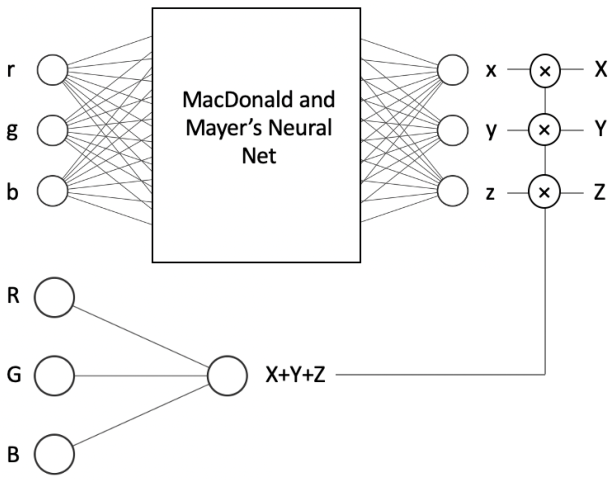
\includegraphics[scale=0.7]{figures/ei_nn.png}}{EI NN}
    \caption{Exposure-Invariant Neural Network. Image from \cite{kucuk2023performance}}
    \label{fig:nn_ei}
\end{figure}

